%==============================================================================
% Figure: E8 Root System Projection (2D)
% Purpose: Visualize E8 lattice structure through 2D projection
% Chapter: Ch03 - Exceptional Lie Groups and Ch04 - E8 Lattice Theory
% Type: Mathematical projection / Symmetry visualization
%==============================================================================

\begin{figure}[htbp]
  \centering
  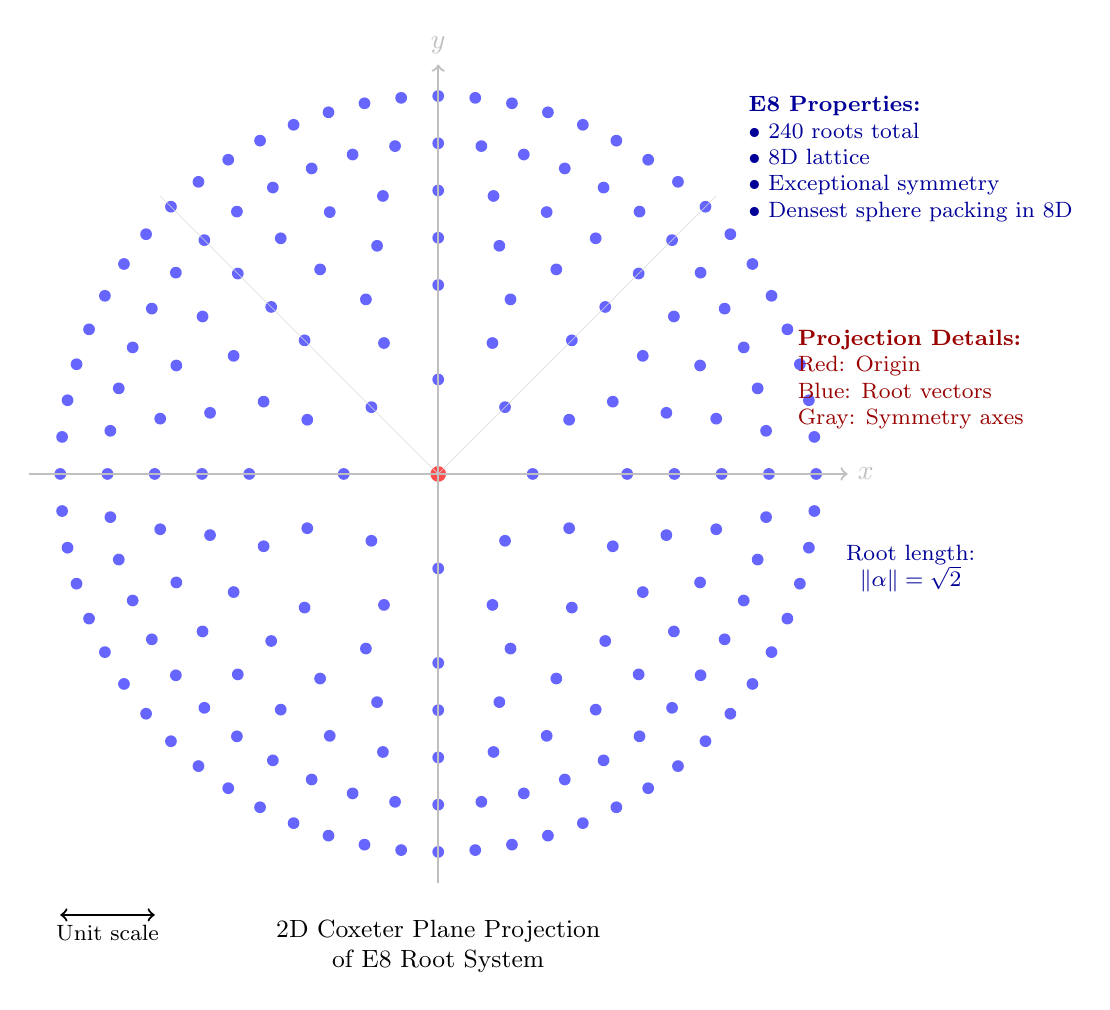
\begin{tikzpicture}[
    scale=0.4,
    root/.style={
      circle,
      fill=blue!60,
      inner sep=1.5pt
    },
    highlight/.style={
      circle,
      fill=red!70,
      inner sep=2pt
    }
  ]

    % E8 root system projected onto 2D (simplified Coxeter plane projection)
    % Using 240 roots projected - showing representative structure

    % Central vertex
    \node[highlight] at (0,0) {};

    % First shell (8-fold symmetry - representative of E8 structure)
    \foreach \angle in {0,45,90,135,180,225,270,315} {
      \node[root] at (\angle:3) {};
    }

    % Second shell (8-fold with offset)
    \foreach \angle in {22.5,67.5,112.5,157.5,202.5,247.5,292.5,337.5} {
      \node[root] at (\angle:4.5) {};
    }

    % Third shell (16-fold)
    \foreach \angle in {0,22.5,45,67.5,90,112.5,135,157.5,180,202.5,225,247.5,270,292.5,315,337.5} {
      \node[root] at (\angle:6) {};
    }

    % Fourth shell (24-fold - showing increased density)
    \foreach \angle in {0,15,30,45,60,75,90,105,120,135,150,165,180,195,210,225,240,255,270,285,300,315,330,345} {
      \node[root] at (\angle:7.5) {};
    }

    % Fifth shell (32-fold)
    \foreach \i in {0,...,31} {
      \pgfmathsetmacro{\angle}{360/32*\i}
      \node[root] at (\angle:9) {};
    }

    % Sixth shell (48-fold)
    \foreach \i in {0,...,47} {
      \pgfmathsetmacro{\angle}{360/48*\i}
      \node[root] at (\angle:10.5) {};
    }

    % Seventh shell (outer ring - 64-fold)
    \foreach \i in {0,...,63} {
      \pgfmathsetmacro{\angle}{360/64*\i}
      \node[root] at (\angle:12) {};
    }

    % Add symmetry lines (8-fold symmetry axes)
    \foreach \angle in {0,45,90,135} {
      \draw[gray!30, very thin] (0,0) -- (\angle:12.5);
    }

    % Coordinate axes
    \draw[->, thick, gray!50] (-13,0) -- (13,0) node[right] {$x$};
    \draw[->, thick, gray!50] (0,-13) -- (0,13) node[above] {$y$};

    % Annotations
    \node[font=\small, align=center] at (0,-15) {
      2D Coxeter Plane Projection\\
      of E8 Root System
    };

    \node[font=\footnotesize, align=left, text=blue!60!black] at (15,10) {
      \textbf{E8 Properties:}\\
      $\bullet$ 240 roots total\\
      $\bullet$ 8D lattice\\
      $\bullet$ Exceptional symmetry\\
      $\bullet$ Densest sphere packing in 8D
    };

    \node[font=\footnotesize, align=left, text=red!60!black] at (15,3) {
      \textbf{Projection Details:}\\
      Red: Origin\\
      Blue: Root vectors\\
      Gray: Symmetry axes
    };

    \node[font=\footnotesize, align=center, text=blue!60!black] at (15,-3) {
      Root length:\\
      $\|\alpha\| = \sqrt{2}$
    };

    % Scale indicator
    \draw[<->, thick] (-12,-14) -- (-9,-14) node[midway, below, font=\footnotesize] {Unit scale};

  \end{tikzpicture}

  \caption{Two-dimensional Coxeter plane projection of the E8 root system. The full E8 lattice exists in 8 dimensions with 240 roots, forming the densest sphere packing in 8D space. This projection reveals the exceptional 8-fold symmetry structure. Each blue dot represents a root vector; shells of increasing radius show the hierarchical organization. The E8 lattice appears in string theory compactifications and provides geometric foundations for grand unification theories. Note: This is a schematic representation; actual root positions involve irrational coordinates in higher dimensions.}
  \label{fig:e8-roots-2d}
\end{figure}
